\chapter{Опис додатків з використанням кросс-платформених рішень}
\label{ch2}


\section{Структура проекту в React Native}
\label{sec:rn_structure_app}

\begin{lstlisting}[style=light, language=Python,label={lst:rn_app_structure},caption=React Native App Layout]
├── App.js (1)
├── Readme.md
├── __tests__ (2)
│ └── App.js
├── android (3)
│ ├── app
│ ├── build
│ ├── build.gradle
│ ├── gradle
│ ├── gradle.properties
│ ├── gradlew
│ ├── gradlew.bat
│ ├── local.properties
│ └── settings.gradle
├── app.json (5)
├── babel.config.js (6)
├── index.js (7)
├── ios (4)
│ ├── BreedRN
│ ├── BreedRN.xcodeproj
│ ├── BreedRN.xcworkspace
│ ├── Podfile
│ ├── Podfile.lock
│ └── Pods
├── metro.config.js (8)
├── node_modules (11)
├── package-lock.json (10)
└── package.json (9)
\end{lstlisting}

\begin{enumerate}
    \item \textbf{App.js} сирцевий код нашого додатку
    \item \textbf{\_\_tests\_\_} сирцевий код тестів
    \item \textbf{android} сирцевий код платформи Android
    \item \textbf{ios} сирцевий код платформи iOS
    \item \textbf{app.json} конфігурує назву додатка піктограму, схеми глибоких зв’язків та ключів API для використання деякими службами
    \item \textbf{babel.config.js} конфігурує Babel - це набір інструментів, який використовується для перетворення коду ECMAScript 2015+ у зворотну сумісну версію JavaScript у поточних та старих браузерах або середовищах.
    \item \textbf{index.js} точка входу для React Native з цього файлу Javascript Engine вивантажує в пам'ять логіку додатку
    \item \textbf{metro.config.js} конфігурує Metro пакувальник JavaScript для платформ Android та iOS
    \item \textbf{package.json} конфігурує дерево залежностей або бібліотек, що використовує проєкт
    \item \textbf{package-lock.json} файл що описує дерево залежностей та відтворюване середовище
    \item \textbf{node\_modules} репозиторій артефактів або сирцевого коду всіх Javascript пакетів, що використовує проєкт
\end{enumerate}


\section{Структура проекту в Flutter}
\label{sec:flutter_structure_app}

\begin{lstlisting}[style=light, language=Python,label={lst:flutter_project_layout},caption=Flutter Project Layout]
├── README.md
├── android (1)
│ ├── app
│ ├── build.gradle
│ ├── gradle
│ ├── gradle.properties
│ ├── gradlew
│ ├── gradlew.bat
│ ├── local.properties
│ └── settings.gradle
├── build (2)
├── ios (3)
│ ├── Flutter
│ ├── Podfile
│ ├── Runner
│ ├── Runner.xcodeproj
│ └── Runner.xcworkspace
├── lib (4)
│ ├── breed_list.dart
│ ├── data
│ ├── domain
│ ├── home.dart
│ ├── main.dart
│ └── presentation
├── pubspec.lock (5)
├── pubspec.yaml (6)
├── test (7)
│ ├── breed_database_test.dart
│ ├── breed_list_view_model_test.dart
│ ├── breed_list_view_model_test.mocks.dart
│ └── network_test.dart
└── web (8)
    ├── favicon.png
    ├── icons
    ├── index.html
    └── manifest.json
\end{lstlisting}

\begin{enumerate}
    \item \textbf{android} сирцевий код платформного коду Android.
    \item \textbf{build} тека з тимчасовими файлами згенерованими Flutter CLI під час побудування проєкту.
    \item \textbf{ios} сирцевий код платформного коду iOS.
    \item \textbf{lib} сирцевий код Flutter, що є серцем репозиторію та описує логіку проєкту.
    \item \textbf{pubspec.lock} файл що описує дерево залежностей та відтворюває середовище.
    \item \textbf{pubspec.yaml} конфігурує дерево залежностей або бібліотек, що використовує проєкт.
    \item \textbf{test} сирцевий код тестів для платформи Flutter.
    \item \textbf{web} сирцевий код платформного для вебсторінки.
\end{enumerate}


\section{Структура проекту Kotlin Multi-Platform}
\label{sec:kmm_structure_app}

\begin{lstlisting}[style=light, language=Python,label={lst:kmm_project_layout},caption=KMM Project Layout]
├── app (1)
│ ├── build.gradle.kts
│ └── src
├── build.gradle.kts
├── buildSrc (2)
│ ├── build.gradle.kts
│ └── src
├── gradle
├── gradle.properties
├── gradlew
├── gradlew.bat
├── ios (3)
│ ├── Podfile
│ ├── Podfile.lock
│ ├── Pods
│ ├── bai_dialog_ios
│ ├── bai_dialog_ios.xcodeproj
│ ├── bai_dialog_ios.xcworkspace
│ ├── bai_dialog_iosTests
│ └── bai_dialog_iosUITests
├── local.properties
├── settings.gradle.kts
└── shared (4)
    ├── build.gradle.kts
    ├── consumer-rules.pro
    ├── proguard-rules.pro
    ├── shared.podspec
    └── src
        ├── androidMain (5)
        ├── androidTest (6)
        ├── commonMain (7)
        ├── commonTest (8)
        ├── iosMain (9)
        ├── iosTest (10)
        └── main (11)
\end{lstlisting}

\begin{enumerate}
    \item \textbf{app} сирцевий код UI імплементації для Android.
    \item \textbf{buildSrc} сирцевий код, що розширює систему розгортання Gradle.
    \item \textbf{ios} сирцевий код UI імплементації для iOS.
    \item \textbf{shared} тека в котрій зберігається загальний код.
    \item \textbf{androidMain} імплементація коду специфічного для Android платформи.
    \item \textbf{androidTest} імплементація тестів специфічних для Android платформи.
    \item \textbf{commonMain} сирцевий код спільної незалежної від платформи логіки.
    \item \textbf{commonTest} імплементація тестів для спільної незалежної від платформи логіки.
    \item \textbf{iosMain} імплементація коду специфічного для iOS платформи.
    \item \textbf{iosTest} імплементація тестів специфічних для iOS платформи.
    \item \textbf{main} репозиторій в якому зберігається код Android модуля, а саме статичні ресурси та AndroidManifest.
\end{enumerate}


\section{Архітектура додатків}
\label{sec:general_app_architecture}

Задача всіх додатків для всіх платформ - це висвітлення списку порід собак з використанням ресурсу https://dog.ceo/api.
Серед поставлених задач було реалізація, як рівня комунікації з мережею, так і рівня взаємодії збереження
даних. Додатково було зроблено рішення підтримувати можливість реєстрації породи в списку улюблених.

Поведінка всіх додатків наслідує послідовність дій описану на мал. \ref{fig:gen_app_flow}.

Загальна архітектура побудована на базі підходу "чистої архітектури" (мал. \ref{fig:clean_architecture}).
Ідеологія архітектури, це організація коду по шарах абстракції \textbf{domain, presentation, data}.

\textbf{Рівень презентації} (або presentation) відповідає за зображення даних. Це дерево віджетів,
що додаток відображуємо на сторінці.

\textbf{Рівень даних} (або data) відповідає за виклики до мережі, збереження даних в БД та робота з файловою системою.

\FloatBarrier

\begin{figure}[ht]
    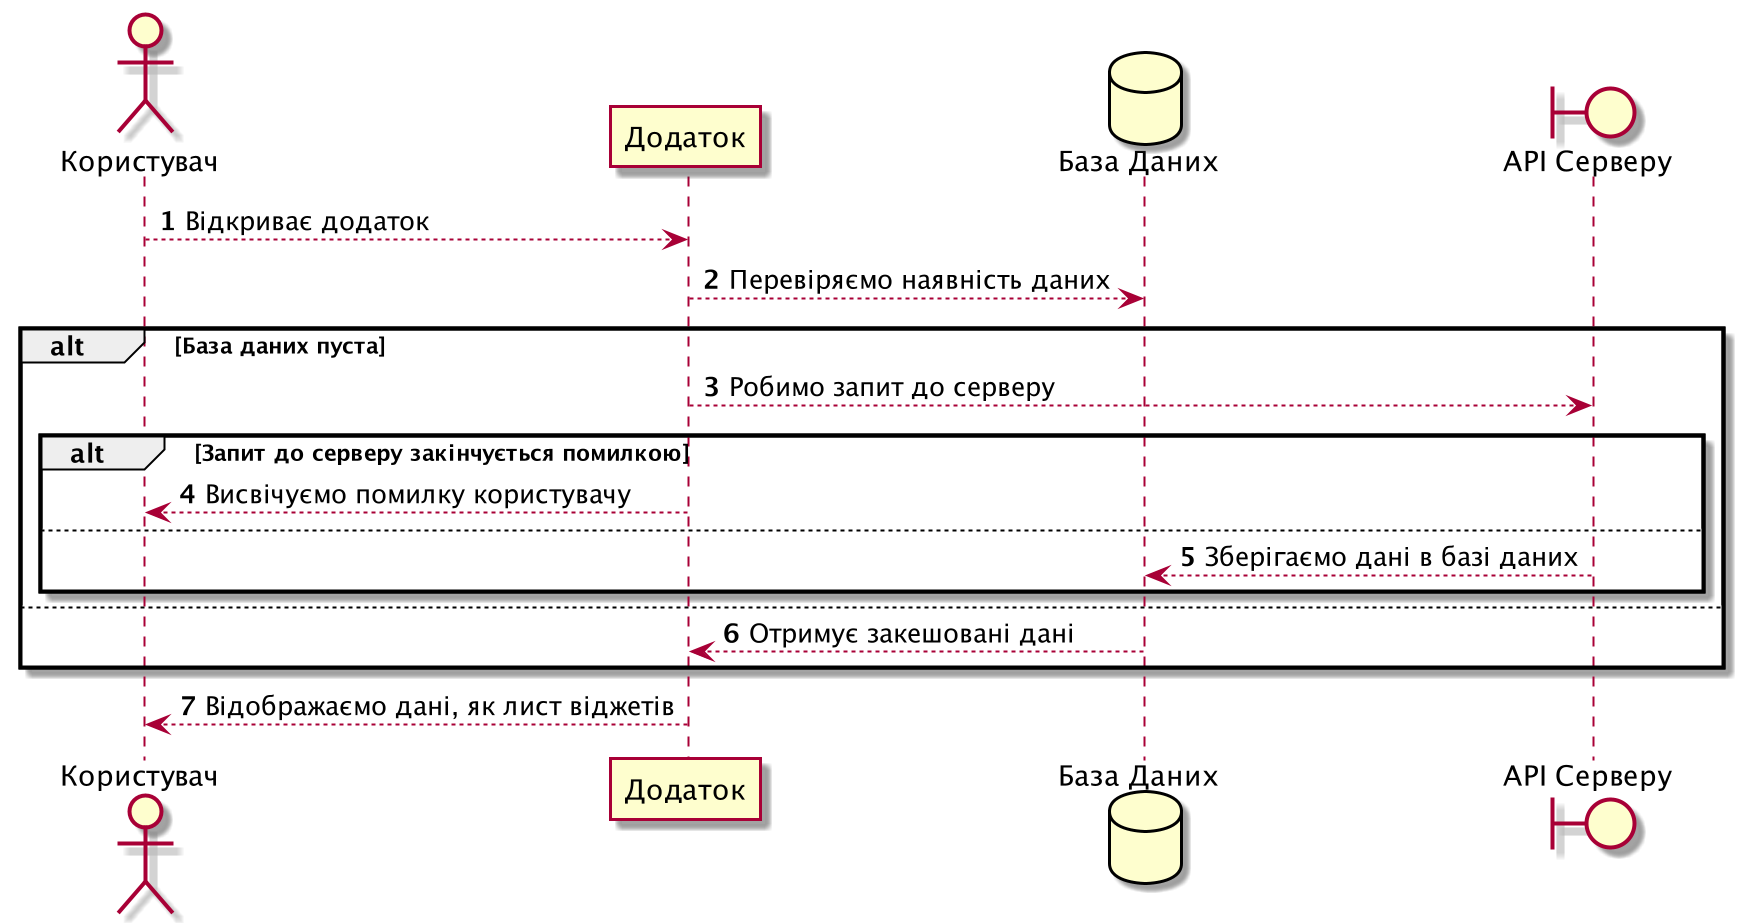
\includegraphics[width=\textwidth]{general_app_flow.png}
    \caption{Загальна схема послідовностей додатку}
    \label{fig:gen_app_flow}
\end{figure}

\textbf{Рівень домену} (або domain) рівень бізнес-логіки. На цьому рівні я визначив контракт. Далі на базі контракту
збудував рівень презентації.

\begin{figure}[h]
    \begin{center}
        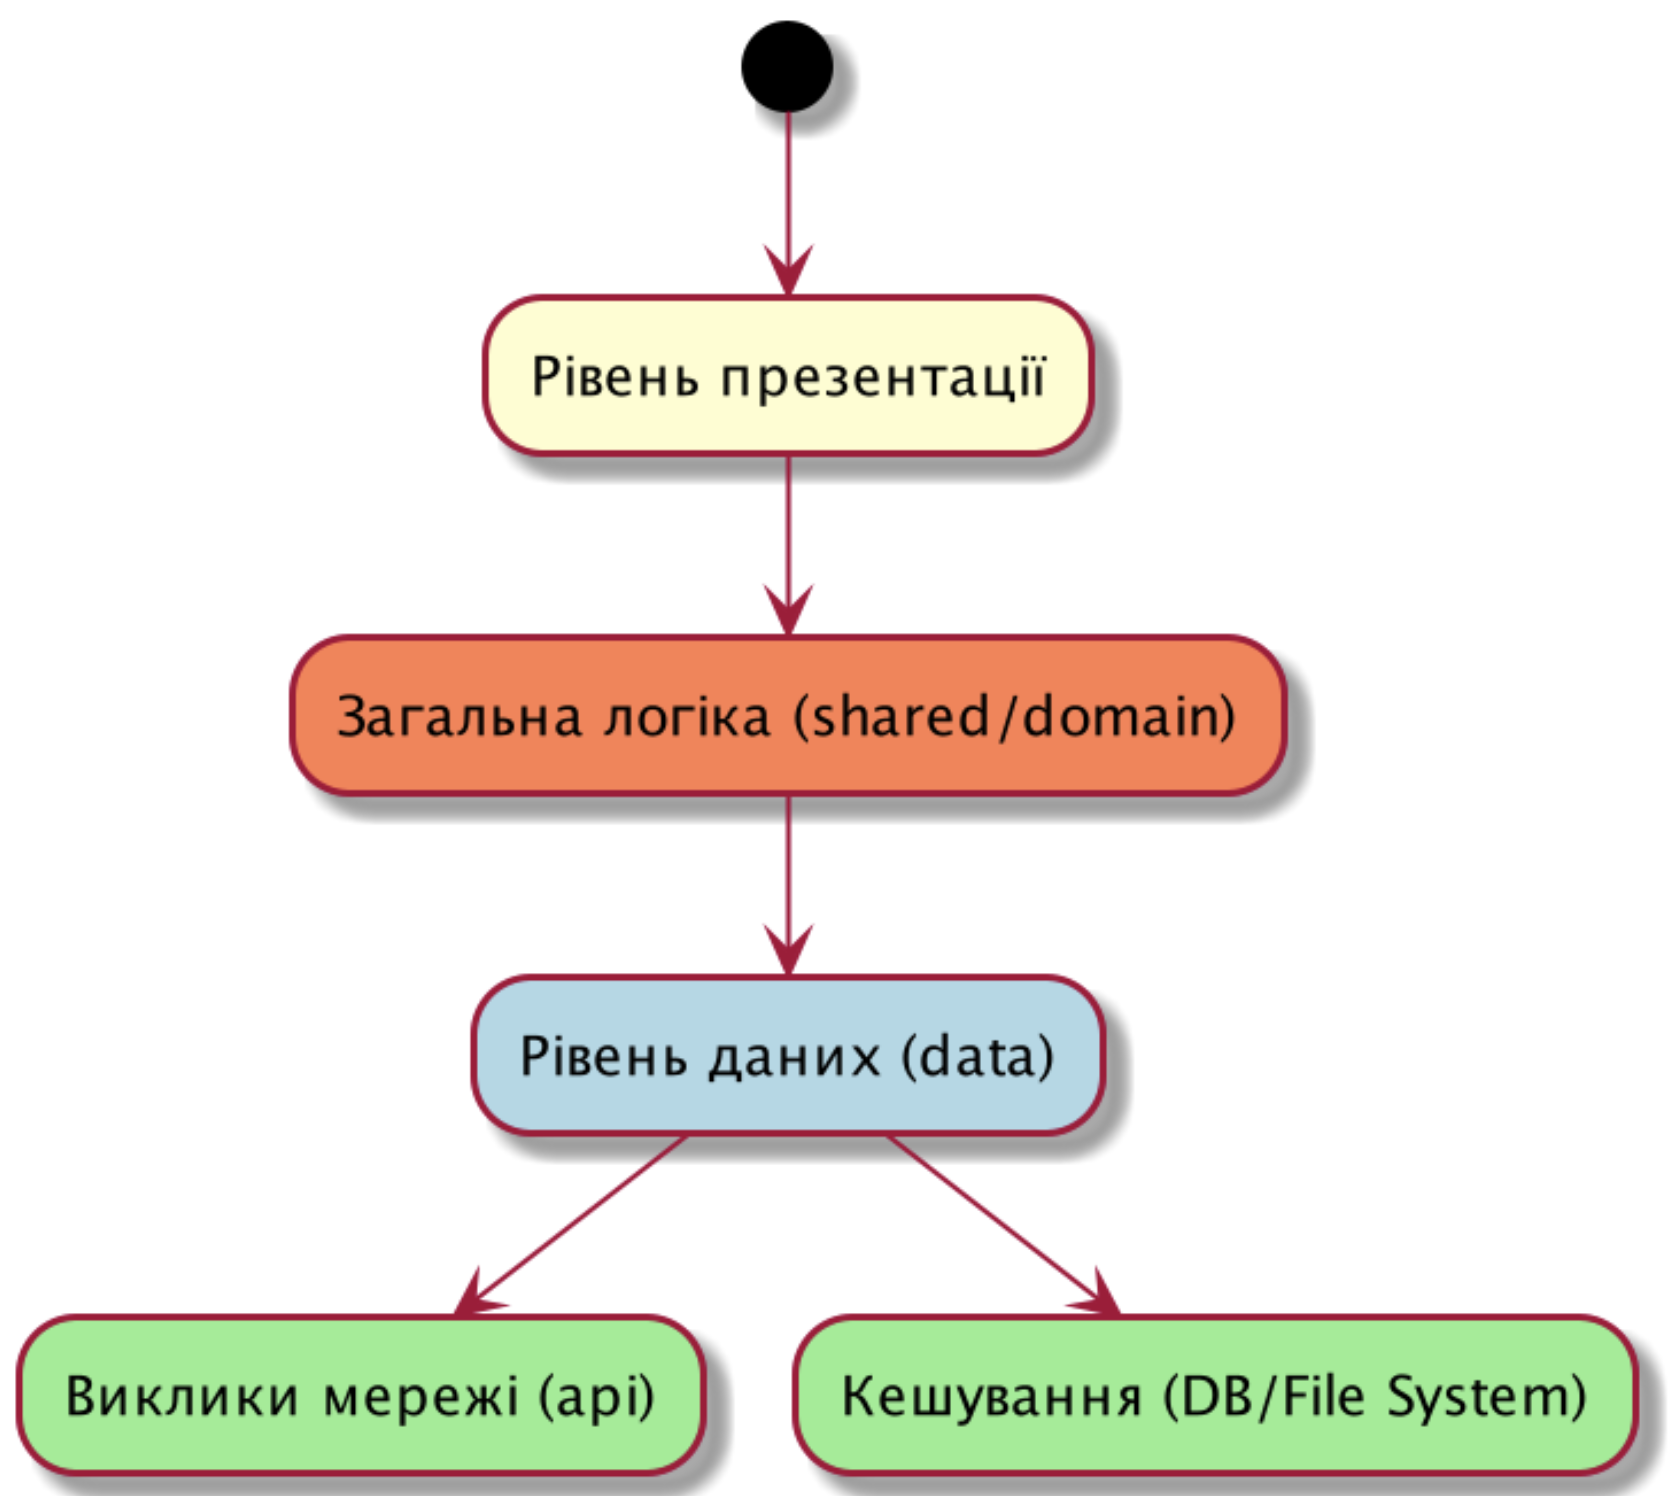
\includegraphics[scale=0.45]{clean_architecture.png}
    \end{center}
    \caption{Чиста архітектура (Clean Architecture)}
    \label{fig:clean_architecture}
\end{figure}

Всі додатки імітують архітектуру MVVM(Model-View-View Model) (див. мал. \ref{fig:gen_app_architecture}).
\textbf{ViewModel} - це контролер, що відповідає за комунікацію з Model рівнем та повертає структуру даних адаптовану під рівень презентації.
\textbf{Model} - це рівень, котрий описує формат рівню даних. На Model рівню я описую контракт взаємодії з даними, як з
мережею так і з базою даних.
\textbf{View} - відповідає за зображення даних і є "пасивним" спостерігачем даних з рівня ViewModel.

\FloatBarrier
\begin{figure}[h]
    \begin{center}
        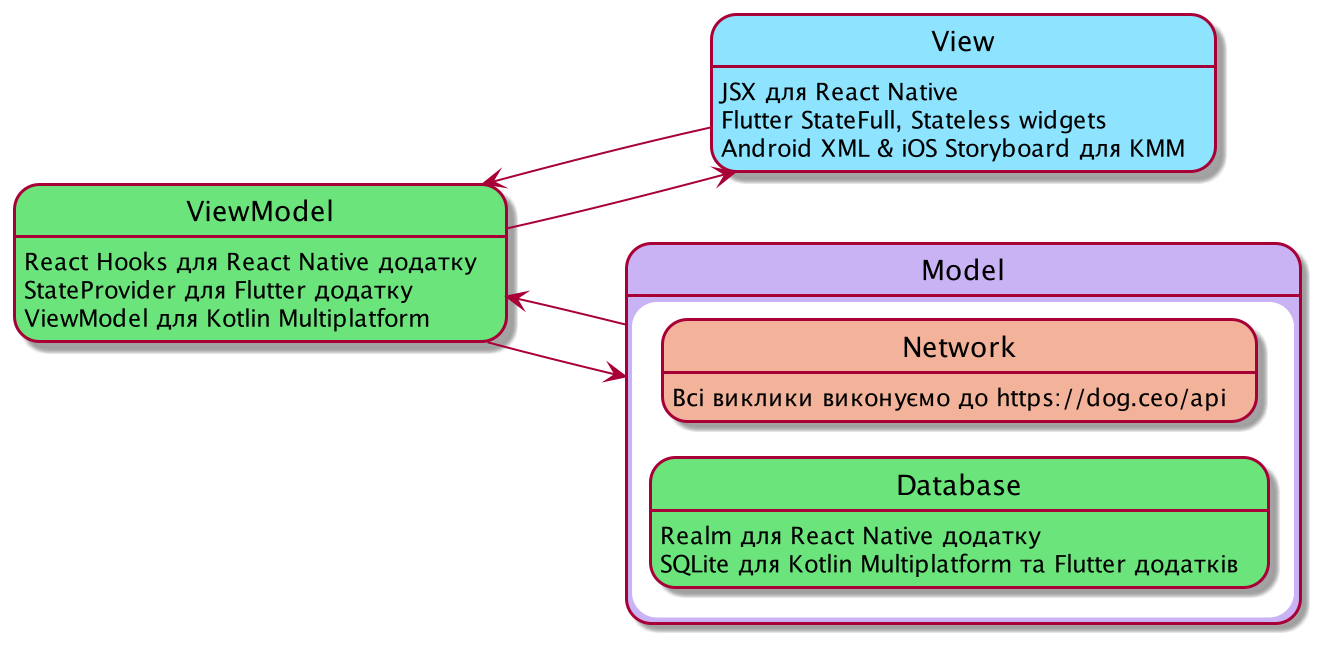
\includegraphics[scale=0.3]{app_layers.png}
    \end{center}
    \caption{Загальна архітектура додатку}
    \label{fig:gen_app_architecture}
\end{figure}
\FloatBarrier


\section{Особливості архітектури додатку React Native}
\label{sec:kn_app_architecture}
В реалізації додатку React Native я використав систему звротніх викликів або так званих "хуків".
Наприклад, \textbf{useState} - це Хук, що дозволяє додавати стан React до функціональних компонентів.

"useState" оголошує "змінну стану" та повертає пару значень: поточний стан та функцію, яка його оновлює.
Наша змінна називається, data, але її можна назвати як завгодно, наприклад banana \ref{lst:rn_state_hooks}.

Використовуючи useEffect хук, я повідомляю React, що наш компонент повинен виконати додаткову фунцію після рендерингу.
React запам'ятає передану нами функцію (яку я буду називати "ефектом") і викличе її пізніше після оновлення UI нашого додатку.

Ефект котрий я створив буде виконаний при ініціалізації додатку
і як результат виконання додаток отримує дані з локальної бази для відображення (див. на \ref{fig:rn_realm})).

\begin{figure}
    \begin{center}
        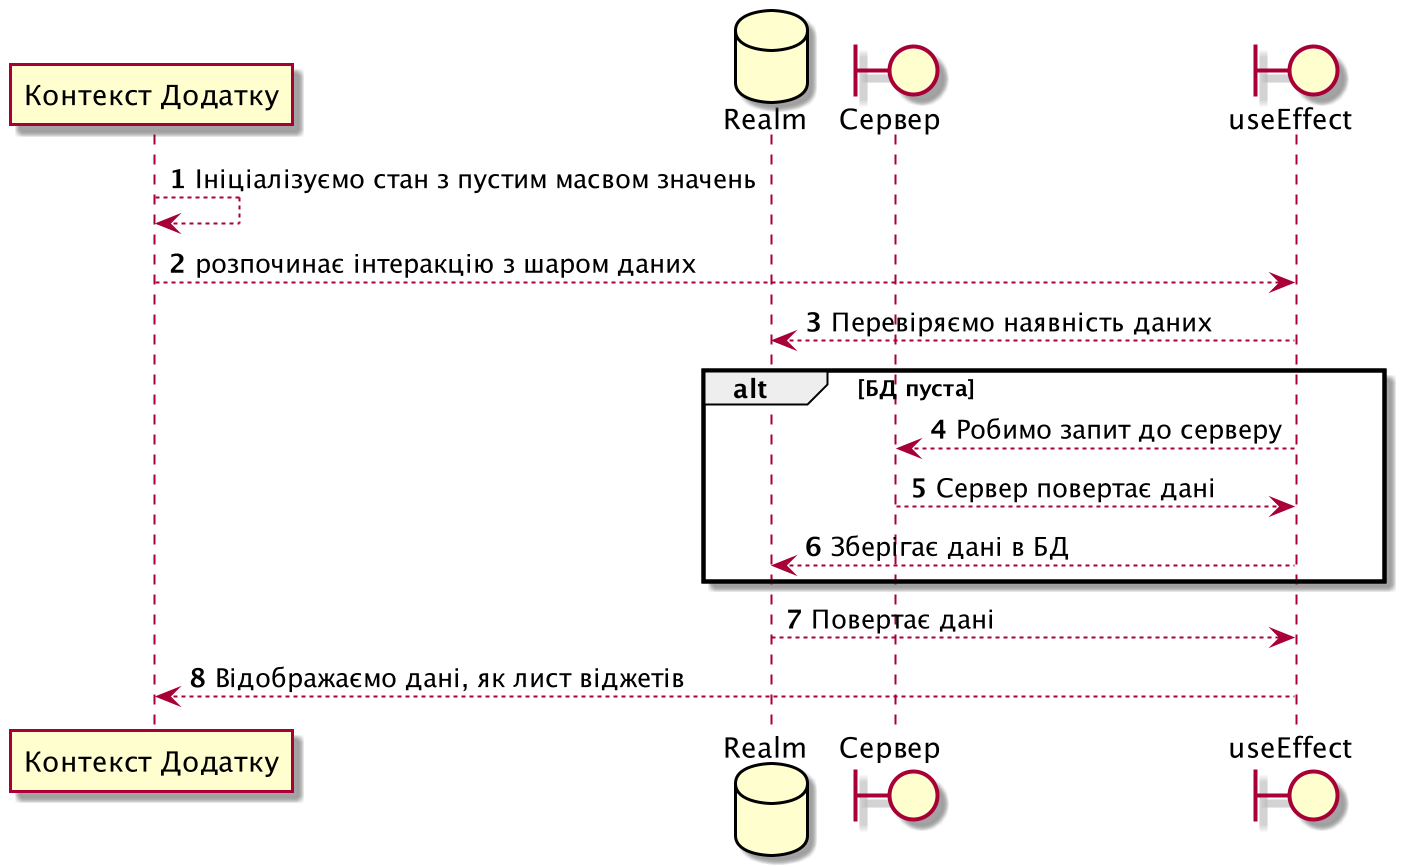
\includegraphics[scale=0.3]{app_widget.png}
        \caption{Взаємодія шарів абстракції в React Native}
        \label{fig:rn_realm}
    \end{center}
\end{figure}


\section{Особливості архітектури додатку Flutter}
\label{sec:flutter_network_app}

Архітектура додатку Flutter наслідує підхід "чистої архітектури" (мал. \ref{fig:clean_architecture}).
На мал. \ref{fig:flutter_classes} показано дерево взаємодії класів, де я позначив залежність класу
від конкретного рівня абстракції на базі розшарування з (presentation, domain, data).

До \textbf{рівня презентації (presentation)} належать віджети Main, MyApp, HomePage, BreedList, BreedItem та
BreedListState, BreedListViewModel, що відповідають за логіку комунікації з інформаційним та доменними рівнями.

До \textbf{рівня домену (domain)} належить Breed (див. рис. \ref{fig:flutter_breed_class}), що описує всю необхідну інформацію таку, як назва породи та, чи
належить вона до списку улюблених. Об'єкти класу Breed це "чиста"(немає залежностей від сторонніх бібліотек) структуру даних і не пов'язані на пряму
з конкретикою реалізації рівня даних. Даний підхід дозволяє мені замінити деталі реалізації рівня даних без впливу на
рівень презентації. Наприклад, я можу замість зберігання даних в БД використати кеш на файловій системі.

\begin{figure}[h]
    \begin{center}
        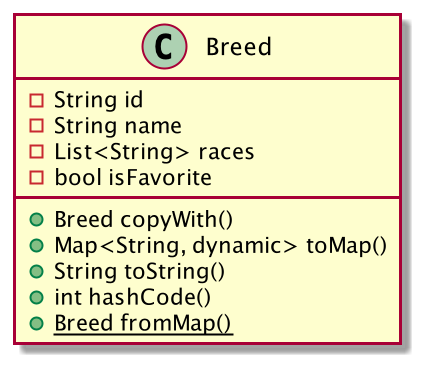
\includegraphics[scale=0.4]{breed_dart.png}
    \end{center}
    \caption{Реалізація структури класу Breed}
    \label{fig:flutter_breed_class}
\end{figure}
\FloatBarrier

До \textbf{рівня даних (data)} належить BreedApi та BreedDatabase. На цьому рівні описана взаємодія з БД та мережею.
BreedApi, як згадувалось в секції \ref{subsec:flutter_http_dart_theory} реалізовано за допомогою пакету \textbf{http/http.dart}.
BreedDatabase реалізовано за допомогою пакету \textbf{SQFlite}, котрий комунікує з локальною SQLite БД. БД використовується
для зберігання інформації про породи собак та додатково зберігає інформацію о всіх улюблених породах собак.

\begin{figure}
    \begin{center}
        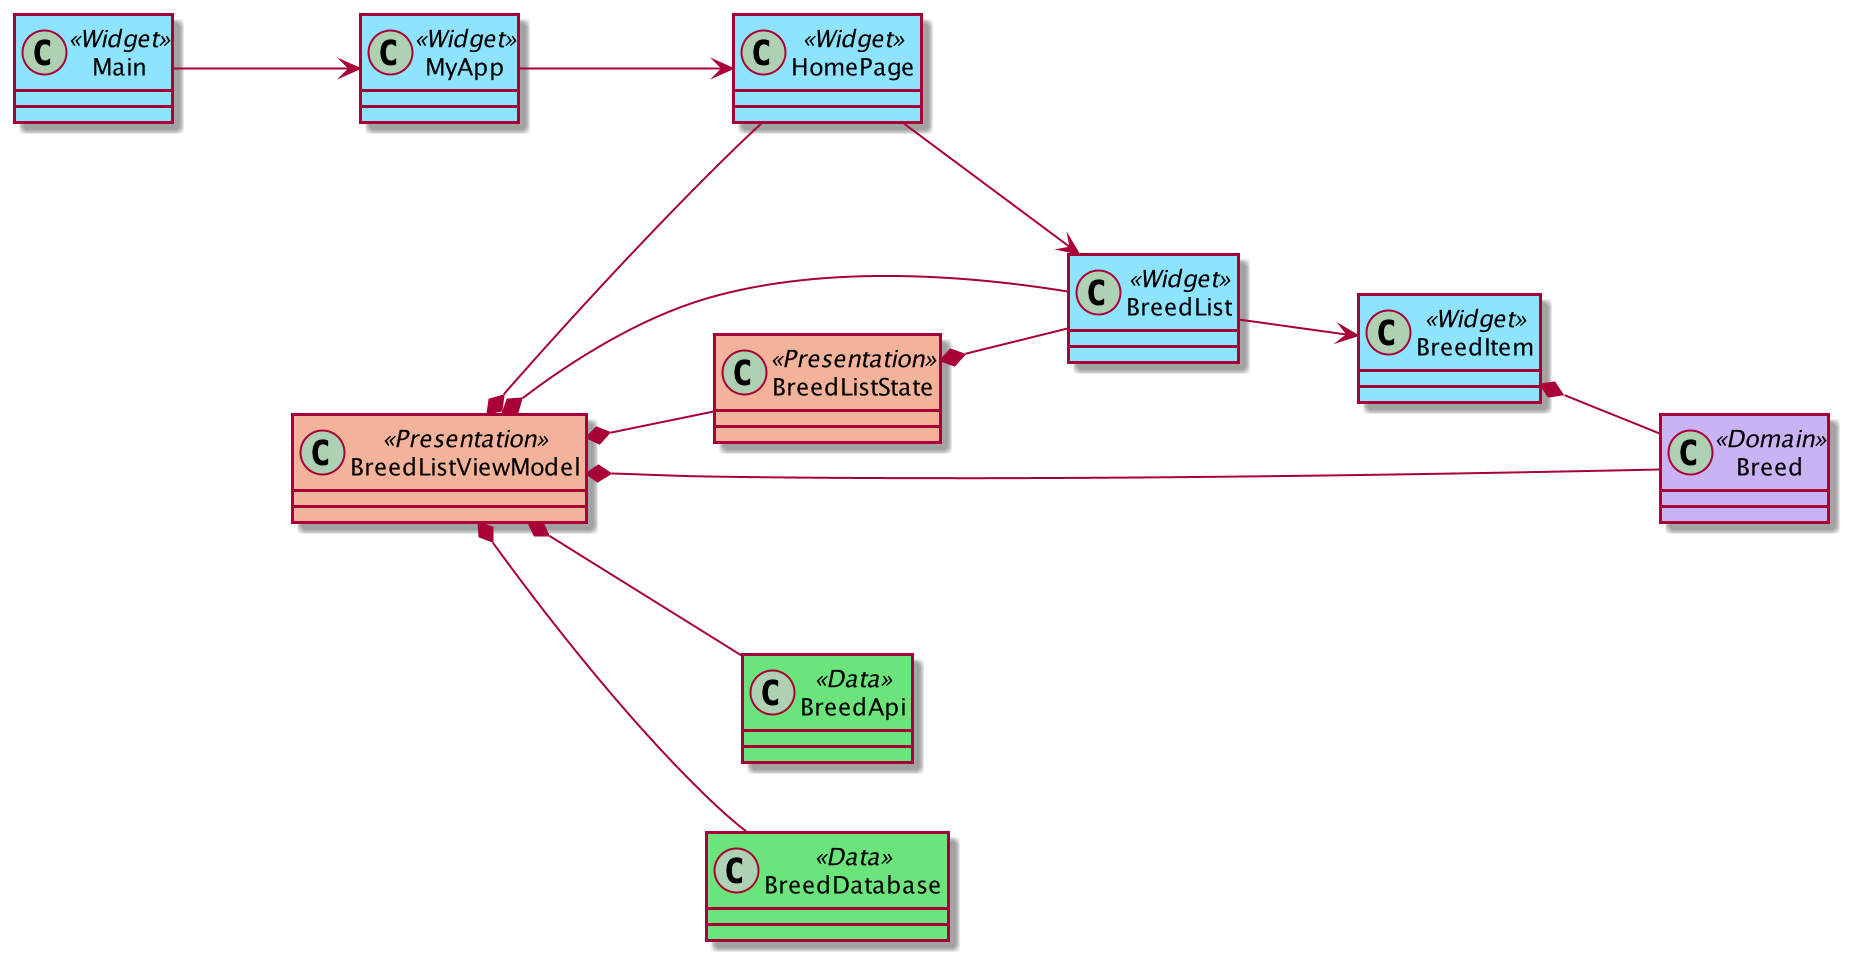
\includegraphics[scale=0.55, width=\textwidth]{flutter_classes.png}
    \end{center}
    \caption{Діаграма класів Flutter}
    \label{fig:flutter_classes}
\end{figure}


\section{Особливості архітектури додатку Kotlin Multiplatform}
\label{sec:kmm_architecture}

Проєкт, незалежно від того, працює він в Android або iOS, використовує базові компоненти презентації
Activity для Android та ViewController для iOS платформ.

Компонент презентації створюють BreedModel, конфігурують зворотні виклики(callbacks) та стартують BreedModel.
BreedModel є загальним кодом MultiPlatform.
BreedModel реалізовує кросс-платформний код та посилається на бібліотеку Multiplatform-Settings,
та два допоміжні класи: DogApiImpl (який реалізує KtorApi) і DatabaseHelper.

DatabseHelper та DogApiImpl використовують бібліотеки Multiplatform для отримання даних і повернення їх до BreedModel.
Зауважимо, що BreedModel посилається на інтерфейс KtorApi. Це дає можливість протестувати модель за допомогою Mock(заглушки) Api.

BreedModel підписується на потік змін з бази даних. Таким чином, будь-які зміни в базі даних будуть викликати
зворотний виклик та відновлювати рівень презентації.
Описана модель повертає список собачих порід та показує на рівні презентації.
Модель отримує інформацію з мережі, а потім зберігає дані в базі даних.

Отримаємо наступний приклад описаний на мал. \ref{fig:kmm_architecture}.

\begin{figure}[h]
    \begin{center}
        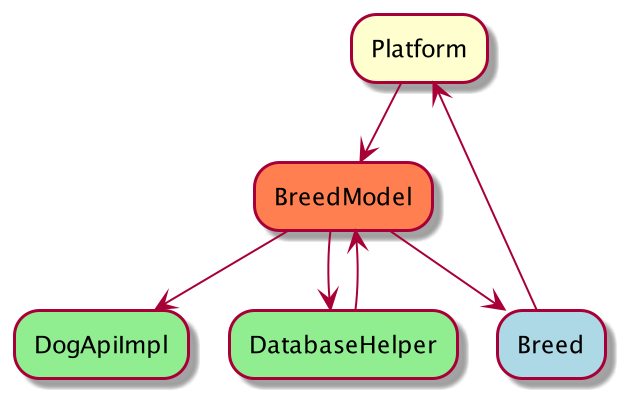
\includegraphics[scale=0.4]{kmm_architecture.png}
    \end{center}
    \caption{Взаємодія шарів абстракції в KMM}
    \label{fig:kmm_architecture}
\end{figure}
\FloatBarrier

Останній пазл нашої конфігурації полягає в використанні багато платформної бібліотеки для зберігання налаштувань (див. мал. \ref{fig:kmm_app_flow}).
В нашому випадку я використовую це рішення для того, щоб зберегти час останньої оновлення, а саме коли було в останнє зроблено запит до сервера.
Коли до BreedModel виконує запит на отримання списку порід з мережі, наша модель спочатку перевіряє, чи виконано це запит протягом минулої години.
Якщо відповідь негативна, то модель приймає вирішення оновити список порід.

\FloatBarrier
\begin{figure}[h]
    \begin{center}
        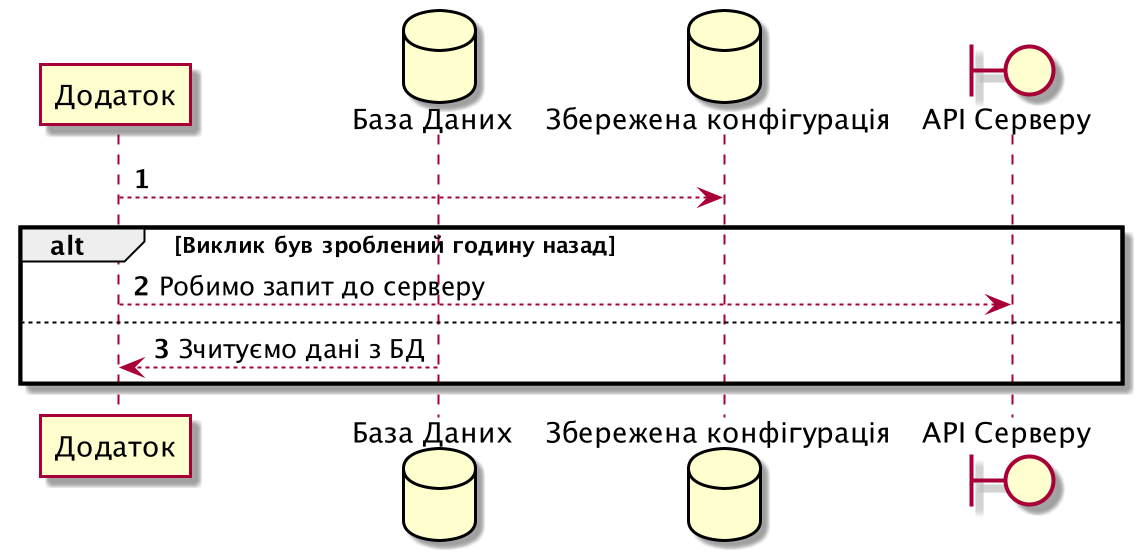
\includegraphics[scale=0.3]{kmm_app_flow.png}
    \end{center}
    \caption{Послідовність дій для перевірки закешовоного стану в KMM}
    \label{fig:kmm_app_flow}
\end{figure}
